\PassOptionsToPackage{unicode=true}{hyperref} % options for packages loaded elsewhere
\PassOptionsToPackage{hyphens}{url}
%
\documentclass[]{article}
\usepackage{lmodern}
\usepackage{amssymb,amsmath}
\usepackage{ifxetex,ifluatex}
\usepackage{fixltx2e} % provides \textsubscript
\ifnum 0\ifxetex 1\fi\ifluatex 1\fi=0 % if pdftex
  \usepackage[T1]{fontenc}
  \usepackage[utf8]{inputenc}
  \usepackage{textcomp} % provides euro and other symbols
\else % if luatex or xelatex
  \usepackage{unicode-math}
  \defaultfontfeatures{Ligatures=TeX,Scale=MatchLowercase}
\fi
% use upquote if available, for straight quotes in verbatim environments
\IfFileExists{upquote.sty}{\usepackage{upquote}}{}
% use microtype if available
\IfFileExists{microtype.sty}{%
\usepackage[]{microtype}
\UseMicrotypeSet[protrusion]{basicmath} % disable protrusion for tt fonts
}{}
\IfFileExists{parskip.sty}{%
\usepackage{parskip}
}{% else
\setlength{\parindent}{0pt}
\setlength{\parskip}{6pt plus 2pt minus 1pt}
}
\usepackage{hyperref}
\hypersetup{
            pdftitle={Project 2},
            pdfauthor={Kathleen Strybos},
            pdfborder={0 0 0},
            breaklinks=true}
\urlstyle{same}  % don't use monospace font for urls
\usepackage[margin=1in]{geometry}
\usepackage{color}
\usepackage{fancyvrb}
\newcommand{\VerbBar}{|}
\newcommand{\VERB}{\Verb[commandchars=\\\{\}]}
\DefineVerbatimEnvironment{Highlighting}{Verbatim}{commandchars=\\\{\}}
% Add ',fontsize=\small' for more characters per line
\usepackage{framed}
\definecolor{shadecolor}{RGB}{248,248,248}
\newenvironment{Shaded}{\begin{snugshade}}{\end{snugshade}}
\newcommand{\AlertTok}[1]{\textcolor[rgb]{0.94,0.16,0.16}{#1}}
\newcommand{\AnnotationTok}[1]{\textcolor[rgb]{0.56,0.35,0.01}{\textbf{\textit{#1}}}}
\newcommand{\AttributeTok}[1]{\textcolor[rgb]{0.77,0.63,0.00}{#1}}
\newcommand{\BaseNTok}[1]{\textcolor[rgb]{0.00,0.00,0.81}{#1}}
\newcommand{\BuiltInTok}[1]{#1}
\newcommand{\CharTok}[1]{\textcolor[rgb]{0.31,0.60,0.02}{#1}}
\newcommand{\CommentTok}[1]{\textcolor[rgb]{0.56,0.35,0.01}{\textit{#1}}}
\newcommand{\CommentVarTok}[1]{\textcolor[rgb]{0.56,0.35,0.01}{\textbf{\textit{#1}}}}
\newcommand{\ConstantTok}[1]{\textcolor[rgb]{0.00,0.00,0.00}{#1}}
\newcommand{\ControlFlowTok}[1]{\textcolor[rgb]{0.13,0.29,0.53}{\textbf{#1}}}
\newcommand{\DataTypeTok}[1]{\textcolor[rgb]{0.13,0.29,0.53}{#1}}
\newcommand{\DecValTok}[1]{\textcolor[rgb]{0.00,0.00,0.81}{#1}}
\newcommand{\DocumentationTok}[1]{\textcolor[rgb]{0.56,0.35,0.01}{\textbf{\textit{#1}}}}
\newcommand{\ErrorTok}[1]{\textcolor[rgb]{0.64,0.00,0.00}{\textbf{#1}}}
\newcommand{\ExtensionTok}[1]{#1}
\newcommand{\FloatTok}[1]{\textcolor[rgb]{0.00,0.00,0.81}{#1}}
\newcommand{\FunctionTok}[1]{\textcolor[rgb]{0.00,0.00,0.00}{#1}}
\newcommand{\ImportTok}[1]{#1}
\newcommand{\InformationTok}[1]{\textcolor[rgb]{0.56,0.35,0.01}{\textbf{\textit{#1}}}}
\newcommand{\KeywordTok}[1]{\textcolor[rgb]{0.13,0.29,0.53}{\textbf{#1}}}
\newcommand{\NormalTok}[1]{#1}
\newcommand{\OperatorTok}[1]{\textcolor[rgb]{0.81,0.36,0.00}{\textbf{#1}}}
\newcommand{\OtherTok}[1]{\textcolor[rgb]{0.56,0.35,0.01}{#1}}
\newcommand{\PreprocessorTok}[1]{\textcolor[rgb]{0.56,0.35,0.01}{\textit{#1}}}
\newcommand{\RegionMarkerTok}[1]{#1}
\newcommand{\SpecialCharTok}[1]{\textcolor[rgb]{0.00,0.00,0.00}{#1}}
\newcommand{\SpecialStringTok}[1]{\textcolor[rgb]{0.31,0.60,0.02}{#1}}
\newcommand{\StringTok}[1]{\textcolor[rgb]{0.31,0.60,0.02}{#1}}
\newcommand{\VariableTok}[1]{\textcolor[rgb]{0.00,0.00,0.00}{#1}}
\newcommand{\VerbatimStringTok}[1]{\textcolor[rgb]{0.31,0.60,0.02}{#1}}
\newcommand{\WarningTok}[1]{\textcolor[rgb]{0.56,0.35,0.01}{\textbf{\textit{#1}}}}
\usepackage{graphicx,grffile}
\makeatletter
\def\maxwidth{\ifdim\Gin@nat@width>\linewidth\linewidth\else\Gin@nat@width\fi}
\def\maxheight{\ifdim\Gin@nat@height>\textheight\textheight\else\Gin@nat@height\fi}
\makeatother
% Scale images if necessary, so that they will not overflow the page
% margins by default, and it is still possible to overwrite the defaults
% using explicit options in \includegraphics[width, height, ...]{}
\setkeys{Gin}{width=\maxwidth,height=\maxheight,keepaspectratio}
\setlength{\emergencystretch}{3em}  % prevent overfull lines
\providecommand{\tightlist}{%
  \setlength{\itemsep}{0pt}\setlength{\parskip}{0pt}}
\setcounter{secnumdepth}{0}
% Redefines (sub)paragraphs to behave more like sections
\ifx\paragraph\undefined\else
\let\oldparagraph\paragraph
\renewcommand{\paragraph}[1]{\oldparagraph{#1}\mbox{}}
\fi
\ifx\subparagraph\undefined\else
\let\oldsubparagraph\subparagraph
\renewcommand{\subparagraph}[1]{\oldsubparagraph{#1}\mbox{}}
\fi

% set default figure placement to htbp
\makeatletter
\def\fps@figure{htbp}
\makeatother


\title{Project 2}
\author{Kathleen Strybos}
\date{4/20/2020}

\begin{document}
\maketitle

\#\#\#Project 2: Modeling, Testing and Predicting on Data for Food
Insecurity in Texas Counties

\#Introduction

\emph{The dataset that was chosen for this project is centered around
health across counties in Texas. The dataset contains 12 different
variables for different health measures across counties in Texas. A few
of these variables include average life expectancy, the rate of diabetes
prevalence, rates of both food insecurity across the county and the rate
of limited food access in the counties, average household incomes,
free/reduced lunch rates among school-aged children, urbanization status
indicators of whether the counties are rural or urban, and the border
status of the counties, which indicates whether or not they are on the
border. This data was acquired at the County Health Rankings and
Roadmaps website and funded by the Robert Wood Johnson Foundation
Program. Overall there are 254 observations, to signify how many
counties there are in Texas.}

\#MANOVA

\begin{Shaded}
\begin{Highlighting}[]
\KeywordTok{library}\NormalTok{(tidyverse)}
\KeywordTok{library}\NormalTok{(dplyr)}
\KeywordTok{library}\NormalTok{(ggplot2)}
\KeywordTok{library}\NormalTok{(lmtest)}
\KeywordTok{library}\NormalTok{(sandwich)}
\KeywordTok{library}\NormalTok{(plotROC)}
\NormalTok{joindata<-}\KeywordTok{read_csv}\NormalTok{(}\StringTok{"joindata.csv"}\NormalTok{)}

\CommentTok{#MANOVA}

\NormalTok{man1<-}\KeywordTok{manova}\NormalTok{(}\KeywordTok{cbind}\NormalTok{(lifeexpectancy,foodinsecurerate, diabeticrate,limitedaccessfoodrate, }
\NormalTok{  Household.Income, free_reduced_lunch_percent,}
\NormalTok{  costpermeal)}\OperatorTok{~}\NormalTok{urbanization, }\DataTypeTok{data=}\NormalTok{joindata)}
\KeywordTok{summary}\NormalTok{(man1)}
\end{Highlighting}
\end{Shaded}

\begin{verbatim}
##               Df  Pillai approx F num Df den Df    Pr(>F)    
## urbanization   1 0.32767   15.874      7    228 < 2.2e-16 ***
## Residuals    234                                             
## ---
## Signif. codes:  0 '***' 0.001 '**' 0.01 '*' 0.05 '.' 0.1 ' ' 1
\end{verbatim}

\begin{Shaded}
\begin{Highlighting}[]
\CommentTok{#Homogeneity of Variances}

\NormalTok{covmats<-joindata}\OperatorTok\KeywordTok{group_by}\NormalTok{(urbanization)}\OperatorTok\KeywordTok{drop_na}\NormalTok{()}\OperatorTok\KeywordTok{do}\NormalTok{(}\DataTypeTok{covs=}\KeywordTok{cov}\NormalTok{(.[}\DecValTok{2}\OperatorTok{:}\DecValTok{8}\NormalTok{]))}
\ControlFlowTok{for}\NormalTok{(i }\ControlFlowTok{in} \DecValTok{1}\OperatorTok{:}\DecValTok{3}\NormalTok{)\{}\KeywordTok{print}\NormalTok{(}\KeywordTok{as.character}\NormalTok{(covmats}\OperatorTok{$}\NormalTok{urbanization[i])); }\KeywordTok{print}\NormalTok{(covmats}\OperatorTok{$}\NormalTok{covs[i])\}}
\end{Highlighting}
\end{Shaded}

\begin{verbatim}
## [1] "Rural"
## [[1]]
##                            lifeexpectancy  diabeticrate foodinsecurerate
## lifeexpectancy                 6.35630750 -6.536322e-01       -4.9811102
## diabeticrate                  -0.65363217  2.261165e+00        4.0666946
## foodinsecurerate              -4.98111018  4.066695e+00       18.8661919
## limitedaccessfoodrate          2.63329284 -2.157059e+00       -4.2066192
## free_reduced_lunch_percent    -0.02870968 -1.945706e+00       -5.9684541
## costpermeal                    0.01756598  2.879765e-02        0.1211542
## Household.Income            2513.97620444 -1.113480e+03    -3231.8512778
##                            limitedaccessfoodrate free_reduced_lunch_percent
## lifeexpectancy                      2.633293e+00              -2.870968e-02
## diabeticrate                       -2.157059e+00              -1.945706e+00
## foodinsecurerate                   -4.206619e+00              -5.968454e+00
## limitedaccessfoodrate               6.638014e+01               2.449074e+01
## free_reduced_lunch_percent          2.449074e+01               9.200310e+01
## costpermeal                        -3.053687e-01              -4.528550e-01
## Household.Income                   -1.819561e+04              -4.767283e+04
##                             costpermeal Household.Income
## lifeexpectancy               0.01756598        2513.9762
## diabeticrate                 0.02879765       -1113.4801
## foodinsecurerate             0.12115417       -3231.8513
## limitedaccessfoodrate       -0.30536866      -18195.6123
## free_reduced_lunch_percent  -0.45285505      -47672.8320
## costpermeal                  0.04267863         539.1542
## Household.Income           539.15419564    55909302.1399
## 
## [1] "Urban"
## [[1]]
##                            lifeexpectancy  diabeticrate foodinsecurerate
## lifeexpectancy               5.690944e+00 -1.501944e+00    -3.262778e+00
## diabeticrate                -1.501944e+00  2.294444e+00     2.027778e+00
## foodinsecurerate            -3.262778e+00  2.027778e+00     1.286111e+01
## limitedaccessfoodrate        5.791806e+00  1.431944e+00    -8.847222e-01
## free_reduced_lunch_percent  -5.079444e+00  5.156944e+00     2.415278e+00
## costpermeal                  6.335231e-02 -5.189815e-02     6.832407e-02
## Household.Income             1.363101e+04 -7.869583e+03    -9.214233e+03
##                            limitedaccessfoodrate free_reduced_lunch_percent
## lifeexpectancy                      5.791806e+00              -5.079444e+00
## diabeticrate                        1.431944e+00               5.156944e+00
## foodinsecurerate                   -8.847222e-01               2.415278e+00
## limitedaccessfoodrate               6.959444e+01               4.611944e+01
## free_reduced_lunch_percent          4.611944e+01               2.117944e+02
## costpermeal                        -2.170648e-01              -1.500023e+00
## Household.Income                   -4.476632e+04              -1.697131e+05
##                              costpermeal Household.Income
## lifeexpectancy                0.06335231        13631.010
## diabeticrate                 -0.05189815        -7869.583
## foodinsecurerate              0.06832407        -9214.233
## limitedaccessfoodrate        -0.21706481       -44766.321
## free_reduced_lunch_percent   -1.50002315      -169713.133
## costpermeal                   0.03638994         1321.786
## Household.Income           1321.78619444    195357053.075
## 
## [1] NA
## [[1]]
## NULL
\end{verbatim}

\begin{Shaded}
\begin{Highlighting}[]
\CommentTok{#Multivariate Normality}
\KeywordTok{nrow}\NormalTok{(}\KeywordTok{filter}\NormalTok{(joindata, urbanization}\OperatorTok{==}\StringTok{"Rural"}\NormalTok{))}
\end{Highlighting}
\end{Shaded}

\begin{verbatim}
## [1] 172
\end{verbatim}

\begin{Shaded}
\begin{Highlighting}[]
\KeywordTok{nrow}\NormalTok{(}\KeywordTok{filter}\NormalTok{(joindata, urbanization}\OperatorTok{==}\StringTok{"Urban"}\NormalTok{))}
\end{Highlighting}
\end{Shaded}

\begin{verbatim}
## [1] 82
\end{verbatim}

\begin{Shaded}
\begin{Highlighting}[]
\CommentTok{#ANOVA}
\KeywordTok{summary.aov}\NormalTok{(man1)}
\end{Highlighting}
\end{Shaded}

\begin{verbatim}
##  Response lifeexpectancy :
##               Df  Sum Sq Mean Sq F value   Pr(>F)   
## urbanization   1   52.16  52.164  8.5113 0.003873 **
## Residuals    234 1434.15   6.129                    
## ---
## Signif. codes:  0 '***' 0.001 '**' 0.01 '*' 0.05 '.' 0.1 ' ' 1
## 
##  Response foodinsecurerate :
##               Df Sum Sq Mean Sq F value Pr(>F)
## urbanization   1   13.4  13.446  0.7998 0.3721
## Residuals    234 3934.3  16.813               
## 
##  Response diabeticrate :
##               Df Sum Sq Mean Sq F value   Pr(>F)   
## urbanization   1  23.42 23.4242  10.307 0.001511 **
## Residuals    234 531.77  2.2725                    
## ---
## Signif. codes:  0 '***' 0.001 '**' 0.01 '*' 0.05 '.' 0.1 ' ' 1
## 
##  Response limitedaccessfoodrate :
##               Df  Sum Sq Mean Sq F value Pr(>F)
## urbanization   1    21.8  21.784  0.3228 0.5705
## Residuals    234 15790.1  67.479               
## 
##  Response Household.Income :
##               Df     Sum Sq    Mean Sq F value    Pr(>F)    
## urbanization   1 8.9697e+09 8969747764  86.594 < 2.2e-16 ***
## Residuals    234 2.4239e+10  103583747                      
## ---
## Signif. codes:  0 '***' 0.001 '**' 0.01 '*' 0.05 '.' 0.1 ' ' 1
## 
##  Response free_reduced_lunch_percent :
##               Df  Sum Sq Mean Sq F value    Pr(>F)    
## urbanization   1  4954.7  4954.7  37.265 4.248e-09 ***
## Residuals    234 31112.0   133.0                      
## ---
## Signif. codes:  0 '***' 0.001 '**' 0.01 '*' 0.05 '.' 0.1 ' ' 1
## 
##  Response costpermeal :
##               Df Sum Sq  Mean Sq F value  Pr(>F)  
## urbanization   1 0.1439 0.143912  3.5509 0.06075 .
## Residuals    234 9.4837 0.040529                  
## ---
## Signif. codes:  0 '***' 0.001 '**' 0.01 '*' 0.05 '.' 0.1 ' ' 1
## 
## 18 observations deleted due to missingness
\end{verbatim}

\begin{Shaded}
\begin{Highlighting}[]
\CommentTok{#Probability of at least one Type 1 Error}
\NormalTok{type1overall<-}\DecValTok{1}\OperatorTok{-}\NormalTok{(}\DecValTok{1}\FloatTok{-0.05}\NormalTok{)}\OperatorTok{^}\DecValTok{8}
\NormalTok{type1overall}
\end{Highlighting}
\end{Shaded}

\begin{verbatim}
## [1] 0.3365796
\end{verbatim}

\begin{Shaded}
\begin{Highlighting}[]
\CommentTok{#Bonferroni Correction}
\NormalTok{bonferroni<-}\FloatTok{0.05}\OperatorTok{/}\DecValTok{8}
\NormalTok{bonferroni}
\end{Highlighting}
\end{Shaded}

\begin{verbatim}
## [1] 0.00625
\end{verbatim}

\emph{There is a significant effect, with a p-value of 2.2e-16, in
urbanization when the MANOVA is performed, meaning there is a mean
difference across urbanization status for one or some of the numeric
response variables. However, we cannot decipher which variable is
showing a mean difference with a MANOVA, so univariate ANOVAs were used
to narrow this down. The assumptions for MANOVA that were likely met
include the assumption for multivariate normality because there were 172
samples for Rural counties taken and 82 samples for Urban counties that
were taken, which is more than 25 in each category. Homogeneity of
covariances does not appear to be met because the covariances between
urban and rural counties differ largely in a few areas, with some
univariate and multivariate outliers, but this might be passable for the
MANOVA, as the assumptions are difficult to meet.}

\emph{Univariate ANOVAs were performed to find responses showing a mean
difference across groups, and life expectancy (p-value of 0.003873),
diabetic rate (p-value of 0.001511), household income (p-value of
2.2e-16) and free and reduced lunch percent (p-value of 0.000000004248)
all showed significance, meaning that the mean differences by
urbanization status differed. For an ANOVA, we can assume that the
assumptions of random sampling, normal distribution of the groups and
equal variance of each group have been met, as the sample sizes contain
independent responses for every county in Texas, and each variable
contains more than 25 samples within each group.}

\emph{There was one MANOVA performed, and seven ANOVAs so overall 8
tests were performed.The probability that I made at least one Type-1
error is 0.3365796. The boneferroni adjusted significance level that I
will use to keep the overall type I error rate at .05 is 0.00625. All
four previously significant tests showed a significant difference even
after Bonferroni adjustment for life expectancy, diabetic rate,
household income, and free/reduced lunch percentage, as their p-values
were much smaller than even the Bonferroni adjusted p-value. No Post-Hoc
tests were done because there were only two categories within
``urbanization,'' so it was visible after doing ANOVAs where the
differences were between groups.}

\hypertarget{randomization-test}{%
\subsection{Randomization Test}\label{randomization-test}}

\begin{Shaded}
\begin{Highlighting}[]
\CommentTok{#Mean Difference in Cost Per Meal}
\NormalTok{joindata}\OperatorTok\KeywordTok{group_by}\NormalTok{(urbanization)}\OperatorTok
\StringTok{  }\KeywordTok{summarize}\NormalTok{(}\DataTypeTok{means=}\KeywordTok{mean}\NormalTok{(costpermeal))}\OperatorTok\KeywordTok{summarize}\NormalTok{(}\StringTok{`}\DataTypeTok{mean_diff:}\StringTok{`}\NormalTok{=}\KeywordTok{diff}\NormalTok{(means))}
\end{Highlighting}
\end{Shaded}

\begin{verbatim}
## # A tibble: 1 x 1
##   `mean_diff:`
##          <dbl>
## 1       0.0471
\end{verbatim}

\begin{Shaded}
\begin{Highlighting}[]
\CommentTok{#Permutations}
\KeywordTok{set.seed}\NormalTok{(}\DecValTok{1234}\NormalTok{)}
\NormalTok{rand_dist<-}\KeywordTok{vector}\NormalTok{()}
\ControlFlowTok{for}\NormalTok{(i }\ControlFlowTok{in} \DecValTok{1}\OperatorTok{:}\DecValTok{5000}\NormalTok{)\{}
\NormalTok{new<-}\KeywordTok{data.frame}\NormalTok{(}\DataTypeTok{costpermeal=}\KeywordTok{sample}\NormalTok{(joindata}\OperatorTok{$}\NormalTok{costpermeal),}
  \DataTypeTok{urbanization=}\NormalTok{joindata}\OperatorTok{$}\NormalTok{urbanization)}
\NormalTok{rand_dist[i]<-}\KeywordTok{mean}\NormalTok{(new[new}\OperatorTok{$}\NormalTok{urbanization}\OperatorTok{==}\StringTok{"Urban"}\NormalTok{,]}\OperatorTok{$}\NormalTok{costpermeal)}\OperatorTok{-}
\StringTok{  }\KeywordTok{mean}\NormalTok{(new[new}\OperatorTok{$}\NormalTok{urbanization}\OperatorTok{==}\StringTok{"Rural"}\NormalTok{,]}\OperatorTok{$}\NormalTok{costpermeal)\}}
\KeywordTok{mean}\NormalTok{(rand_dist}\OperatorTok{>}\FloatTok{0.04713556}\OperatorTok{|}\StringTok{ }\NormalTok{rand_dist}\OperatorTok{<}\StringTok{ }\FloatTok{-0.04713556}\NormalTok{)}
\end{Highlighting}
\end{Shaded}

\begin{verbatim}
## [1] 0.0774
\end{verbatim}

\begin{Shaded}
\begin{Highlighting}[]
\CommentTok{#Histogram of the Null Distribution and Test Statistic}
\NormalTok{\{}\KeywordTok{hist}\NormalTok{(rand_dist,}\DataTypeTok{main=}\StringTok{""}\NormalTok{, }\DataTypeTok{ylab =} \StringTok{"Count (n)"}\NormalTok{,); }\KeywordTok{abline}\NormalTok{(}\DataTypeTok{v=}\OperatorTok{-}\FloatTok{0.04713556}\NormalTok{,  }\DataTypeTok{col=}\StringTok{"red"}\NormalTok{); }
  \KeywordTok{abline}\NormalTok{(}\DataTypeTok{v=}\FloatTok{0.04713556}\NormalTok{,  }\DataTypeTok{col=}\StringTok{"red"}\NormalTok{)\}}
\end{Highlighting}
\end{Shaded}

\begin{center}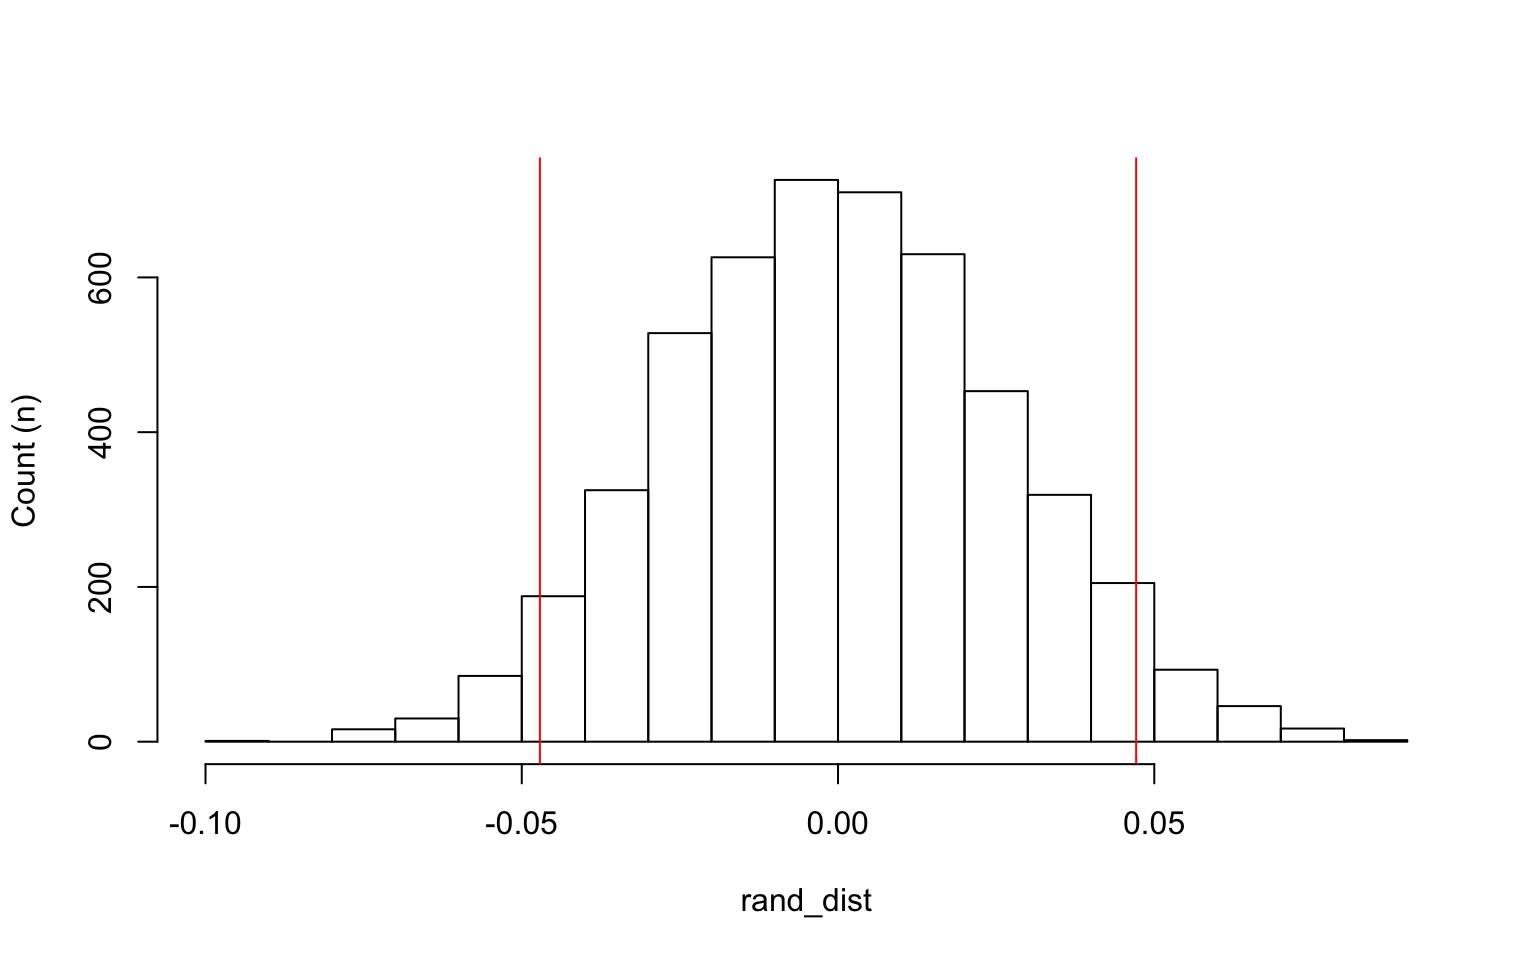
\includegraphics{project2_files/figure-latex/unnamed-chunk-2-1} \end{center}

\begin{Shaded}
\begin{Highlighting}[]
\CommentTok{#Comparison to t-test}
\KeywordTok{t.test}\NormalTok{(}\DataTypeTok{data=}\NormalTok{joindata, costpermeal}\OperatorTok{~}\NormalTok{urbanization)}
\end{Highlighting}
\end{Shaded}

\begin{verbatim}
## 
##  Welch Two Sample t-test
## 
## data:  costpermeal by urbanization
## t = -1.8102, df = 168.89, p-value = 0.07205
## alternative hypothesis: true difference in means is not equal to 0
## 95 percent confidence interval:
##  -0.098540332  0.004269203
## sample estimates:
## mean in group Rural mean in group Urban 
##            2.851279            2.898415
\end{verbatim}

\emph{The null hypothesis of this randomization test is that the mean
cost per meal is the same for urban and rural counties. The alternative
hypothesis is that the mean cost per meal is not the same for urban and
rural counties. The two tailed p-value of the randomization test came
out to be 0.0754, which is not significant in comparison to a reference
of 0.05. Moreover, when a Two Sample t-test was done, the p-value was
0.07205, which is also not significant, indicating that the
randomization test achieved similar results. We can then fail to reject
the null hypothesis that the mean cost per meal is the same for urban
and rural counties, due to a large p-value. The plot of the null
distribution shows the red line at the positive and negative test
statistics, which was 0.04713556. }

\#Linear Regression

\begin{Shaded}
\begin{Highlighting}[]
\CommentTok{#Linear Regression Model}
\NormalTok{joindata}\OperatorTok{$}\NormalTok{foodinsecurerate_c<-joindata}\OperatorTok{$}\NormalTok{foodinsecurerate}\OperatorTok{-}\KeywordTok{mean}\NormalTok{(joindata}\OperatorTok{$}\NormalTok{foodinsecurerate, }
  \DataTypeTok{na.rm=}\NormalTok{T)}
\NormalTok{joindata}\OperatorTok{$}\NormalTok{costpermeal_c<-joindata}\OperatorTok{$}\NormalTok{costpermeal}\OperatorTok{-}\KeywordTok{mean}\NormalTok{(joindata}\OperatorTok{$}\NormalTok{costpermeal, }\DataTypeTok{na.rm=}\NormalTok{T)}
\NormalTok{fit<-}\KeywordTok{lm}\NormalTok{(foodinsecurerate_c }\OperatorTok{~}\StringTok{ }\NormalTok{costpermeal_c }\OperatorTok{*}\StringTok{ }\NormalTok{border_status, }\DataTypeTok{data=}\NormalTok{joindata)}
\KeywordTok{summary}\NormalTok{(fit)}
\end{Highlighting}
\end{Shaded}

\begin{verbatim}
## 
## Call:
## lm(formula = foodinsecurerate_c ~ costpermeal_c * border_status, 
##     data = joindata)
## 
## Residuals:
##     Min      1Q  Median      3Q     Max 
## -8.2732 -2.4593 -0.0027  2.3783 10.3988 
## 
## Coefficients:
##                                       Estimate Std. Error t value Pr(>|t|)    
## (Intercept)                            -4.9538     0.8647  -5.729 2.90e-08 ***
## costpermeal_c                          -0.1617     2.3624  -0.068    0.945    
## border_statusNon-Border                 5.7605     0.8991   6.407 7.32e-10 ***
## costpermeal_c:border_statusNon-Border  -2.5713     2.8136  -0.914    0.362    
## ---
## Signif. codes:  0 '***' 0.001 '**' 0.01 '*' 0.05 '.' 0.1 ' ' 1
## 
## Residual standard error: 3.574 on 250 degrees of freedom
## Multiple R-squared:  0.2246, Adjusted R-squared:  0.2153 
## F-statistic: 24.13 on 3 and 250 DF,  p-value: 9.478e-14
\end{verbatim}

\begin{Shaded}
\begin{Highlighting}[]
\CommentTok{#Regression Plot}
\NormalTok{fit}\OperatorTok\KeywordTok{ggplot}\NormalTok{(}\KeywordTok{aes}\NormalTok{(costpermeal_c, foodinsecurerate_c, }\DataTypeTok{color=}\NormalTok{border_status))}\OperatorTok{+}\KeywordTok{geom_point}\NormalTok{()}\OperatorTok{+}
\StringTok{  }\KeywordTok{geom_smooth}\NormalTok{(}\DataTypeTok{method=}\StringTok{"lm"}\NormalTok{)}\OperatorTok{+}
\StringTok{  }\KeywordTok{ggtitle}\NormalTok{(}\StringTok{"Regression of Food Insecurity Rate by Cost Per Meal"}\NormalTok{)}
\end{Highlighting}
\end{Shaded}

\begin{center}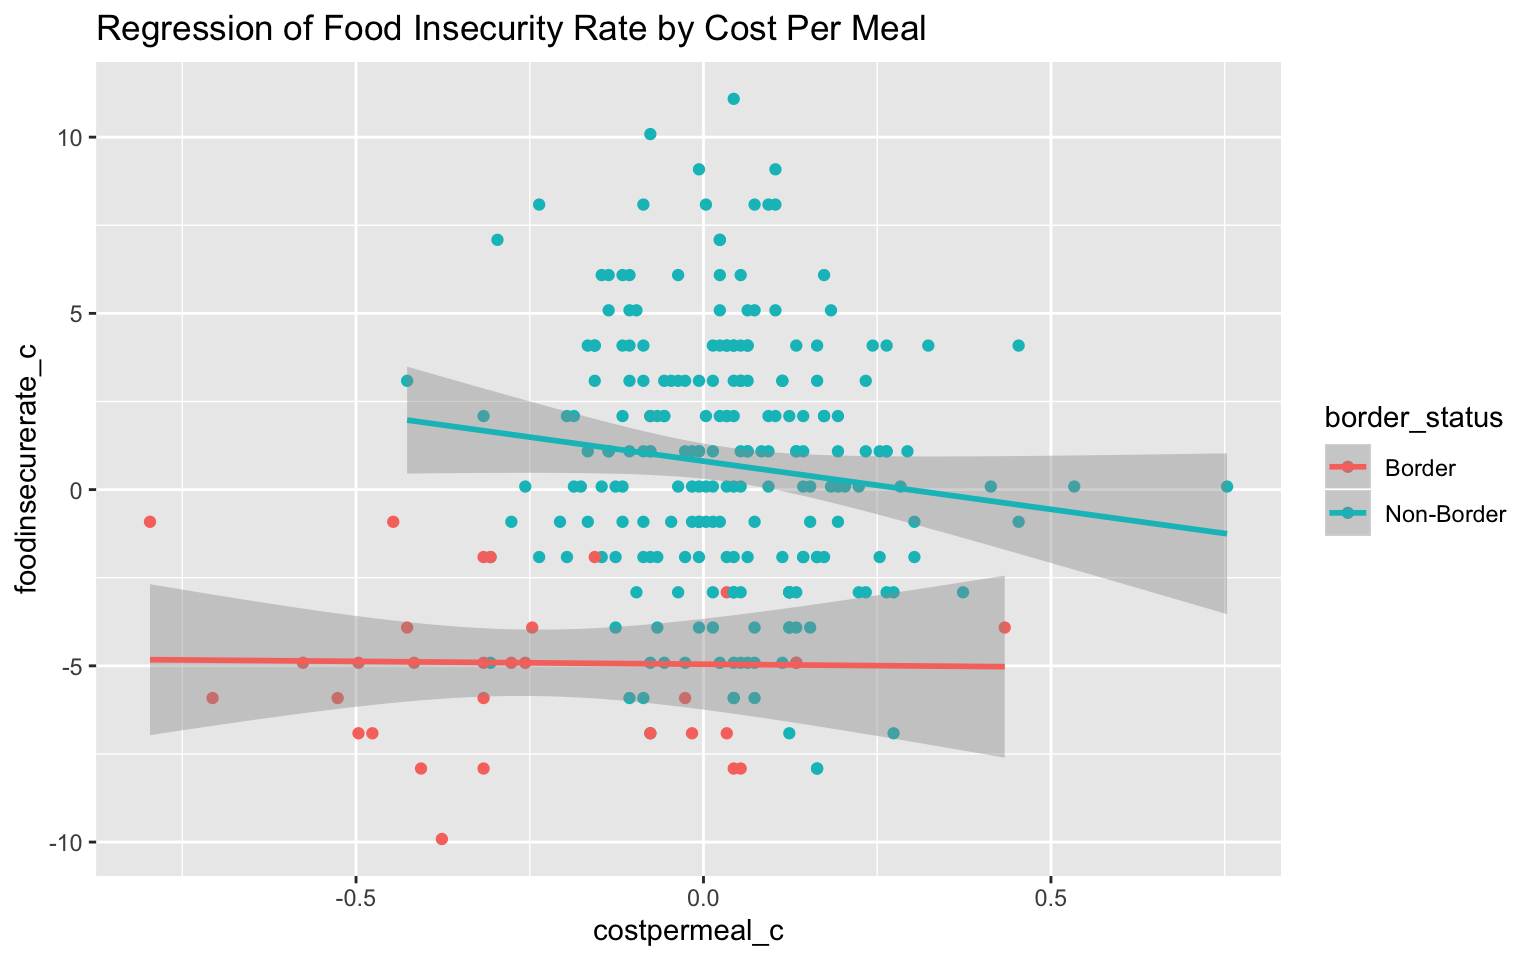
\includegraphics{project2_files/figure-latex/unnamed-chunk-3-1} \end{center}

\begin{Shaded}
\begin{Highlighting}[]
\CommentTok{#Normality Assumption: Data is Normal}
\NormalTok{resids<-}\KeywordTok{lm}\NormalTok{(foodinsecurerate_c}\OperatorTok{~}\NormalTok{costpermeal_c}\OperatorTok{*}\NormalTok{border_status, }\DataTypeTok{data=}\NormalTok{joindata)}\OperatorTok{$}\NormalTok{residuals}
\KeywordTok{ggplot}\NormalTok{()}\OperatorTok{+}\KeywordTok{geom_histogram}\NormalTok{(}\KeywordTok{aes}\NormalTok{(resids),}\DataTypeTok{bins=}\DecValTok{10}\NormalTok{)}\OperatorTok{+}
\StringTok{  }\KeywordTok{ggtitle}\NormalTok{(}\StringTok{"Histogram of Residuals"}\NormalTok{)}
\end{Highlighting}
\end{Shaded}

\begin{center}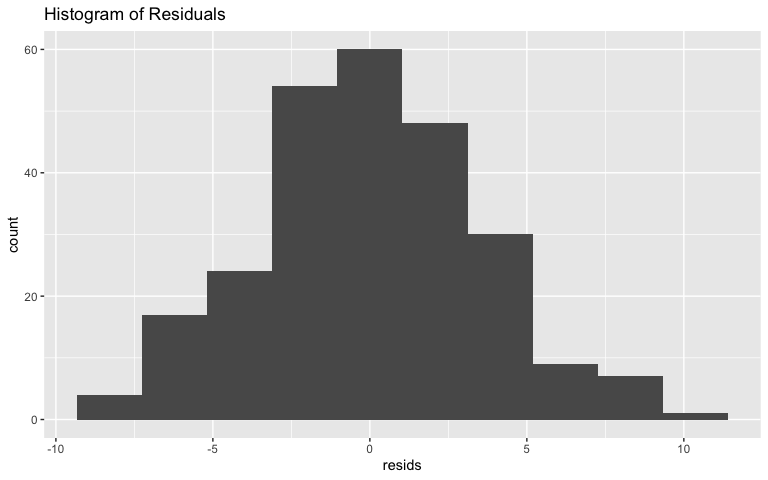
\includegraphics{project2_files/figure-latex/unnamed-chunk-3-2} \end{center}

\begin{Shaded}
\begin{Highlighting}[]
\KeywordTok{ggplot}\NormalTok{()}\OperatorTok{+}\KeywordTok{geom_qq}\NormalTok{(}\KeywordTok{aes}\NormalTok{(}\DataTypeTok{sample=}\NormalTok{resids))}\OperatorTok{+}\KeywordTok{geom_qq}\NormalTok{()}\OperatorTok{+}
\StringTok{  }\KeywordTok{ggtitle}\NormalTok{(}\StringTok{"QQ Plot"}\NormalTok{)}
\end{Highlighting}
\end{Shaded}

\begin{center}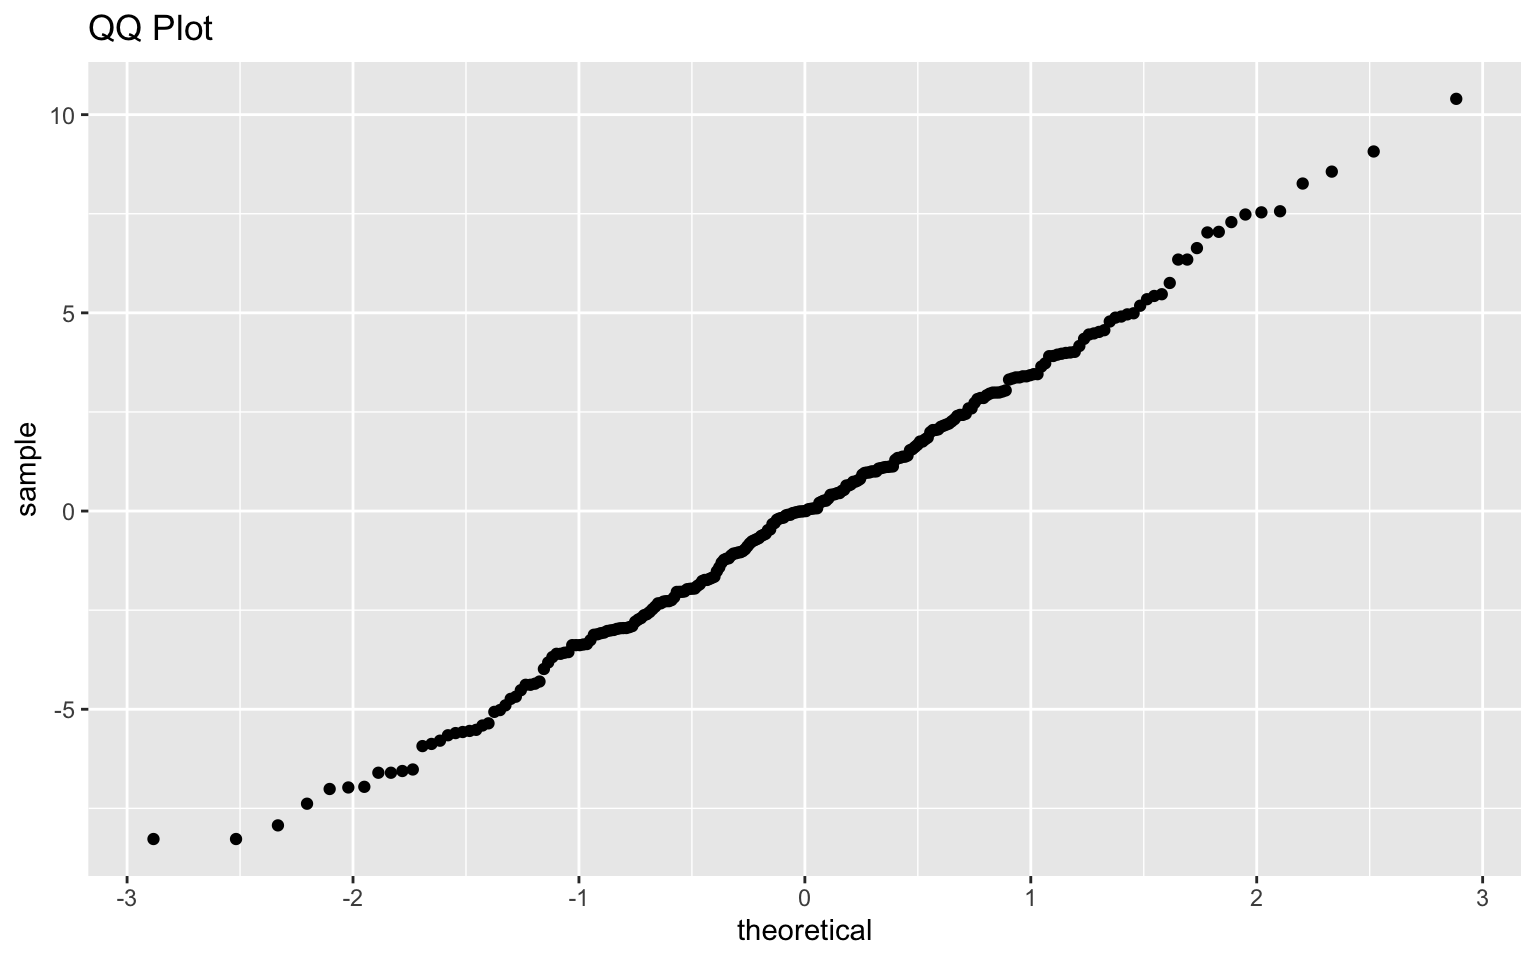
\includegraphics{project2_files/figure-latex/unnamed-chunk-3-3} \end{center}

\begin{Shaded}
\begin{Highlighting}[]
\KeywordTok{shapiro.test}\NormalTok{(resids)}
\end{Highlighting}
\end{Shaded}

\begin{verbatim}
## 
##  Shapiro-Wilk normality test
## 
## data:  resids
## W = 0.9957, p-value = 0.7085
\end{verbatim}

\begin{Shaded}
\begin{Highlighting}[]
\CommentTok{#Linearity Assumption}
\NormalTok{fitted<-}\KeywordTok{lm}\NormalTok{(foodinsecurerate_c}\OperatorTok{~}\NormalTok{costpermeal_c}\OperatorTok{*}\NormalTok{border_status, }\DataTypeTok{data=}\NormalTok{joindata)}\OperatorTok{$}\NormalTok{fitted.values}
\KeywordTok{ggplot}\NormalTok{()}\OperatorTok{+}\KeywordTok{geom_point}\NormalTok{(}\KeywordTok{aes}\NormalTok{(resids,fitted))}\OperatorTok{+}
\StringTok{  }\KeywordTok{ggtitle}\NormalTok{(}\StringTok{"Residuals vs. Fitted Values"}\NormalTok{)}
\end{Highlighting}
\end{Shaded}

\begin{center}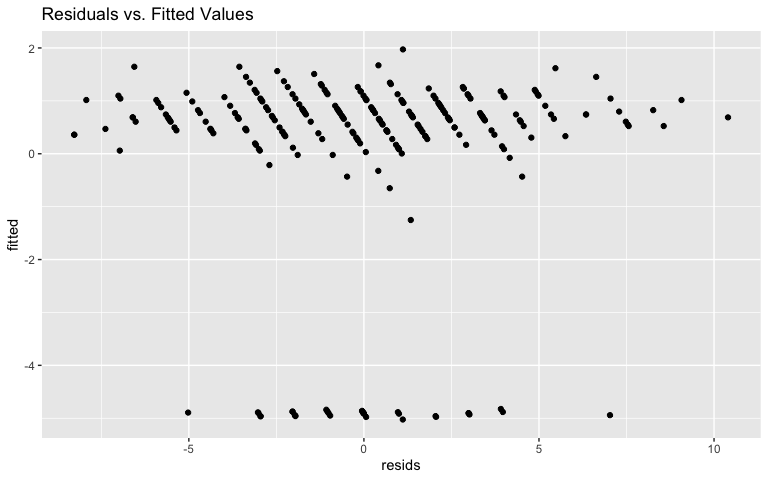
\includegraphics{project2_files/figure-latex/unnamed-chunk-3-4} \end{center}

\begin{Shaded}
\begin{Highlighting}[]
\CommentTok{#Homoskedasticity}
\KeywordTok{bptest}\NormalTok{(fit) }\CommentTok{#Fail to reject the null hypothesis that data is homoskedastic}
\end{Highlighting}
\end{Shaded}

\begin{verbatim}
## 
##  studentized Breusch-Pagan test
## 
## data:  fit
## BP = 5.3442, df = 3, p-value = 0.1483
\end{verbatim}

\begin{Shaded}
\begin{Highlighting}[]
\CommentTok{#Robust Standard Errors: Redo Regression}
\KeywordTok{coeftest}\NormalTok{(fit, }\DataTypeTok{vcov =} \KeywordTok{vcovHC}\NormalTok{(fit))}
\end{Highlighting}
\end{Shaded}

\begin{verbatim}
## 
## t test of coefficients:
## 
##                                       Estimate Std. Error t value  Pr(>|t|)    
## (Intercept)                           -4.95379    0.63103 -7.8503 1.219e-13 ***
## costpermeal_c                         -0.16166    1.70938 -0.0946    0.9247    
## border_statusNon-Border                5.76048    0.68115  8.4569 2.315e-15 ***
## costpermeal_c:border_statusNon-Border -2.57129    2.17218 -1.1837    0.2376    
## ---
## Signif. codes:  0 '***' 0.001 '**' 0.01 '*' 0.05 '.' 0.1 ' ' 1
\end{verbatim}

\begin{Shaded}
\begin{Highlighting}[]
\CommentTok{#Proportion of the Variation Explained}
\KeywordTok{summary}\NormalTok{(fit)}\OperatorTok{$}\NormalTok{r.sq}
\end{Highlighting}
\end{Shaded}

\begin{verbatim}
## [1] 0.2245676
\end{verbatim}

\emph{Predicted food insecurity rate for an average cost per meal at a
border county is 4.9538 percent below the centered mean of the food
insecurity rate. Controlling for border status, for every one dollar
increase in the centered cost per meal, the food insecurity rate
decreases by 0.16166 percent. At an average cost per meal, non-border
counties have a 5.76048 percent higher food insecurity rate as compared
to border counties. The slope for cost per meal on food insecurity rate
is 2.57129 units lower for non-border counties compared to border
counties.}

\emph{The data meets the assumption of normality and homoskedasticity,
and therefore linearity is also met through homoskedasticity. A
Shapiro\_Wilk Normality test was run, along with a histogram and QQ plot
to check for normality, and all results confirmed normality of the data.
The null hypothesis for homoskedasticity fails to be rejected after
running the Breusch-Pagan test, with a p-value of 0.1483, which is
greater than 0.05.}

\emph{After redoing the regression using homoskedastic standard errors,
significance was maintained for the effect of border status when the
cost per meal is controlled for. The standard errors for border status
decreased by about two-tenths from 0.8991 to 0.68115, and the standard
error for cost per meal decreased from 2.3624 to 1.70938. The standard
error for the interaction between border status and cost per meal
decreased slightly from 2.8136 to 2.17218 with robust standard errors.}

\emph{The proportion of the variation in the outcome that the model
explains, or the R-squared value, is 0.2246, or 22.46\%.}

\#Linear Regression with Bootstrapped Standard Errors

\begin{Shaded}
\begin{Highlighting}[]
\NormalTok{fit<-}\KeywordTok{lm}\NormalTok{(foodinsecurerate_c }\OperatorTok{~}\StringTok{ }\NormalTok{costpermeal_c}\OperatorTok{*}\NormalTok{border_status, }\DataTypeTok{data=}\NormalTok{joindata)}
\KeywordTok{summary}\NormalTok{(fit)}
\end{Highlighting}
\end{Shaded}

\begin{verbatim}
## 
## Call:
## lm(formula = foodinsecurerate_c ~ costpermeal_c * border_status, 
##     data = joindata)
## 
## Residuals:
##     Min      1Q  Median      3Q     Max 
## -8.2732 -2.4593 -0.0027  2.3783 10.3988 
## 
## Coefficients:
##                                       Estimate Std. Error t value Pr(>|t|)    
## (Intercept)                            -4.9538     0.8647  -5.729 2.90e-08 ***
## costpermeal_c                          -0.1617     2.3624  -0.068    0.945    
## border_statusNon-Border                 5.7605     0.8991   6.407 7.32e-10 ***
## costpermeal_c:border_statusNon-Border  -2.5713     2.8136  -0.914    0.362    
## ---
## Signif. codes:  0 '***' 0.001 '**' 0.01 '*' 0.05 '.' 0.1 ' ' 1
## 
## Residual standard error: 3.574 on 250 degrees of freedom
## Multiple R-squared:  0.2246, Adjusted R-squared:  0.2153 
## F-statistic: 24.13 on 3 and 250 DF,  p-value: 9.478e-14
\end{verbatim}

\begin{Shaded}
\begin{Highlighting}[]
\CommentTok{#Bootstrapping}
\KeywordTok{set.seed}\NormalTok{(}\DecValTok{1234}\NormalTok{)}
\NormalTok{samp_distn<-}\KeywordTok{replicate}\NormalTok{(}\DecValTok{5000}\NormalTok{, \{}
\NormalTok{boot_dat <-}\StringTok{ }\KeywordTok{sample_frac}\NormalTok{(joindata, }\DataTypeTok{replace=}\NormalTok{T) }
\NormalTok{fit <-}\StringTok{ }\KeywordTok{lm}\NormalTok{(foodinsecurerate_c }\OperatorTok{~}\StringTok{ }\NormalTok{costpermeal_c}\OperatorTok{*}\NormalTok{border_status, }\DataTypeTok{data=}\NormalTok{boot_dat)}
\KeywordTok{coef}\NormalTok{(fit)}
\NormalTok{\})}
\NormalTok{samp_distn }\OperatorTok\StringTok{ }\NormalTok{t }\OperatorTok\StringTok{ }\NormalTok{as.data.frame }\OperatorTok\StringTok{ }\KeywordTok{summarize_all}\NormalTok{(sd)}
\end{Highlighting}
\end{Shaded}

\begin{verbatim}
##   (Intercept) costpermeal_c border_statusNon-Border
## 1   0.6358113      1.635783               0.6828607
##   costpermeal_c:border_statusNon-Border
## 1                              2.110855
\end{verbatim}

\emph{The bootstrapped standard errors shows similar standard errors
that were seen in the robust standard errors of the linear regression,
however they are very different than the original standard errors from
the linear regression. The bootstrapped SE for costpermeal\_c is
1.673076, which is similar to the robust SE of 1.70938, but different
from the original SE of 2.3624. Because the bootstrapped and robust SEs
went down, this means the p-values got smaller as well. The bootstrapped
SE for border status is 0.6910803, which is similar to the robust SE of
0.68115, and smaller than the original SE of 0.8991, meaning the p-value
is smaller for the adjusted SEs. The bootstrapped SE for the interaction
is 2.158202, which is similar to the robust SE of 2.17218, but smaller
than the original SE of 2.8136, meaning the p-value is smaller for the
adjusted SEs too.}

\#Logistic Regression

\begin{Shaded}
\begin{Highlighting}[]
\CommentTok{#Logistic Regression}
\NormalTok{joindata_log<-}\StringTok{ }\NormalTok{joindata}\OperatorTok\KeywordTok{mutate}\NormalTok{(}\DataTypeTok{Urb_binary=}\KeywordTok{ifelse}\NormalTok{(urbanization}\OperatorTok{==}\StringTok{"Urban"}\NormalTok{,}\DecValTok{1}\NormalTok{,}\DecValTok{0}\NormalTok{))}
\NormalTok{fit<-}\KeywordTok{glm}\NormalTok{(Urb_binary }\OperatorTok{~}\StringTok{ }\NormalTok{limitedaccessfoodrate}\OperatorTok{+}\NormalTok{Household.Income, }\DataTypeTok{data=}\NormalTok{joindata_log,}
  \DataTypeTok{family=}\KeywordTok{binomial}\NormalTok{(}\DataTypeTok{link=}\StringTok{"logit"}\NormalTok{))}
\KeywordTok{coeftest}\NormalTok{(fit)}
\end{Highlighting}
\end{Shaded}

\begin{verbatim}
## 
## z test of coefficients:
## 
##                          Estimate  Std. Error z value  Pr(>|z|)    
## (Intercept)           -6.1719e+00  9.1239e-01 -6.7645 1.337e-11 ***
## limitedaccessfoodrate -6.2741e-03  1.6491e-02 -0.3805    0.7036    
## Household.Income       1.0923e-04  1.7054e-05  6.4047 1.507e-10 ***
## ---
## Signif. codes:  0 '***' 0.001 '**' 0.01 '*' 0.05 '.' 0.1 ' ' 1
\end{verbatim}

\begin{Shaded}
\begin{Highlighting}[]
\KeywordTok{exp}\NormalTok{(}\KeywordTok{coef}\NormalTok{(fit))}
\end{Highlighting}
\end{Shaded}

\begin{verbatim}
##           (Intercept) limitedaccessfoodrate      Household.Income 
##           0.002087343           0.993745502           1.000109233
\end{verbatim}

\begin{Shaded}
\begin{Highlighting}[]
\CommentTok{#Confusion Matrix}
\NormalTok{join_conf<-joindata_log}\OperatorTok\KeywordTok{drop_na}\NormalTok{(limitedaccessfoodrate)}\OperatorTok\KeywordTok{mutate}\NormalTok{(}\DataTypeTok{prob=}\KeywordTok{predict}\NormalTok{(fit, }
  \DataTypeTok{type=}\StringTok{"response"}\NormalTok{), }
  \DataTypeTok{prediction=}\KeywordTok{ifelse}\NormalTok{(prob}\OperatorTok{>}\FloatTok{0.5}\NormalTok{,}\DecValTok{1}\NormalTok{,}\DecValTok{0}\NormalTok{))}
\NormalTok{classify<-join_conf}\OperatorTok\KeywordTok{transmute}\NormalTok{(prob,prediction,}\DataTypeTok{truth=}\NormalTok{Urb_binary)}
\NormalTok{classify}
\end{Highlighting}
\end{Shaded}

\begin{verbatim}
## # A tibble: 253 x 3
##     prob prediction truth
##    <dbl>      <dbl> <dbl>
##  1 0.163          0     0
##  2 0.665          1     0
##  3 0.216          0     0
##  4 0.237          0     1
##  5 0.541          1     1
##  6 0.437          0     1
##  7 0.287          0     1
##  8 0.619          1     1
##  9 0.167          0     0
## 10 0.454          0     1
## # ... with 243 more rows
\end{verbatim}

\begin{Shaded}
\begin{Highlighting}[]
\KeywordTok{table}\NormalTok{(}\DataTypeTok{prediction=}\NormalTok{ classify}\OperatorTok{$}\NormalTok{prediction, }\DataTypeTok{truth=}\NormalTok{classify}\OperatorTok{$}\NormalTok{truth)}\OperatorTok\KeywordTok{addmargins}\NormalTok{()}
\end{Highlighting}
\end{Shaded}

\begin{verbatim}
##           truth
## prediction   0   1 Sum
##        0   154  48 202
##        1    17  34  51
##        Sum 171  82 253
\end{verbatim}

\begin{Shaded}
\begin{Highlighting}[]
\CommentTok{#Accuracy}
\NormalTok{(}\DecValTok{154}\OperatorTok{+}\DecValTok{34}\NormalTok{)}\OperatorTok{/}\DecValTok{253}
\end{Highlighting}
\end{Shaded}

\begin{verbatim}
## [1] 0.743083
\end{verbatim}

\begin{Shaded}
\begin{Highlighting}[]
\CommentTok{#Sensitivity (TPR)}
\DecValTok{34}\OperatorTok{/}\DecValTok{82}
\end{Highlighting}
\end{Shaded}

\begin{verbatim}
## [1] 0.4146341
\end{verbatim}

\begin{Shaded}
\begin{Highlighting}[]
\CommentTok{#Specificity (FPR)}
\DecValTok{154}\OperatorTok{/}\DecValTok{171}
\end{Highlighting}
\end{Shaded}

\begin{verbatim}
## [1] 0.9005848
\end{verbatim}

\begin{Shaded}
\begin{Highlighting}[]
\CommentTok{#Precision (PPV)}
\DecValTok{34}\OperatorTok{/}\DecValTok{51}
\end{Highlighting}
\end{Shaded}

\begin{verbatim}
## [1] 0.6666667
\end{verbatim}

\begin{Shaded}
\begin{Highlighting}[]
\CommentTok{#Density Plot of Log-Odds}
\NormalTok{join_conf}\OperatorTok{$}\NormalTok{logit<-}\KeywordTok{predict}\NormalTok{(fit,}\DataTypeTok{type=}\StringTok{"link"}\NormalTok{)}
\NormalTok{join_conf}\OperatorTok\KeywordTok{ggplot}\NormalTok{()}\OperatorTok{+}\KeywordTok{geom_density}\NormalTok{(}\KeywordTok{aes}\NormalTok{(logit,}\DataTypeTok{color=}\NormalTok{urbanization,}\DataTypeTok{fill=}\NormalTok{urbanization), }
  \DataTypeTok{alpha=}\NormalTok{.}\DecValTok{4}\NormalTok{)}\OperatorTok{+}
\StringTok{  }\KeywordTok{theme}\NormalTok{(}\DataTypeTok{legend.position=}\KeywordTok{c}\NormalTok{(.}\DecValTok{85}\NormalTok{,.}\DecValTok{85}\NormalTok{))}\OperatorTok{+}\KeywordTok{geom_vline}\NormalTok{(}\DataTypeTok{xintercept=}\DecValTok{0}\NormalTok{)}\OperatorTok{+}\KeywordTok{xlab}\NormalTok{(}\StringTok{"predictor (logit)"}\NormalTok{)}\OperatorTok{+}
\StringTok{  }\KeywordTok{geom_rug}\NormalTok{(}\KeywordTok{aes}\NormalTok{(logit,}\DataTypeTok{color=}\NormalTok{urbanization)) }\OperatorTok{+}\StringTok{ }\KeywordTok{ggtitle}\NormalTok{(}\StringTok{"Density Plot of Log-Odds"}\NormalTok{) }
\end{Highlighting}
\end{Shaded}

\begin{center}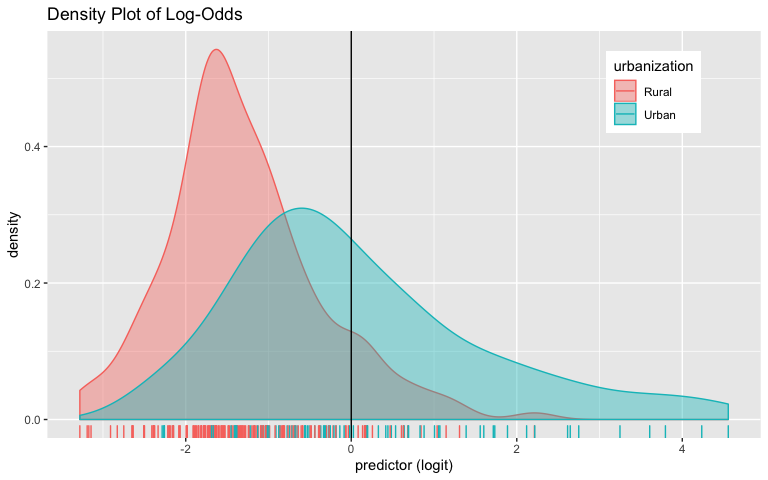
\includegraphics{project2_files/figure-latex/unnamed-chunk-7-1} \end{center}

\begin{Shaded}
\begin{Highlighting}[]
\CommentTok{#ROC Plot}
\KeywordTok{library}\NormalTok{(plotROC)}
\NormalTok{ROCplot<-}\KeywordTok{ggplot}\NormalTok{(classify)}\OperatorTok{+}\KeywordTok{geom_roc}\NormalTok{(}\KeywordTok{aes}\NormalTok{(}\DataTypeTok{d=}\NormalTok{truth,}\DataTypeTok{m=}\NormalTok{prob), }\DataTypeTok{n.cuts=}\DecValTok{0}\NormalTok{)}\OperatorTok{+}\KeywordTok{geom_segment}\NormalTok{(}\KeywordTok{aes}\NormalTok{(}\DataTypeTok{x=}\DecValTok{0}\NormalTok{,}
  \DataTypeTok{xend=}\DecValTok{1}\NormalTok{, }\DataTypeTok{y=}\DecValTok{0}\NormalTok{, }\DataTypeTok{yend=}\DecValTok{1}\NormalTok{), }\DataTypeTok{lty=}\DecValTok{2}\NormalTok{)}\OperatorTok{+}\KeywordTok{ggtitle}\NormalTok{(}\StringTok{"ROC Curve"}\NormalTok{)}
\NormalTok{ROCplot}
\end{Highlighting}
\end{Shaded}

\begin{center}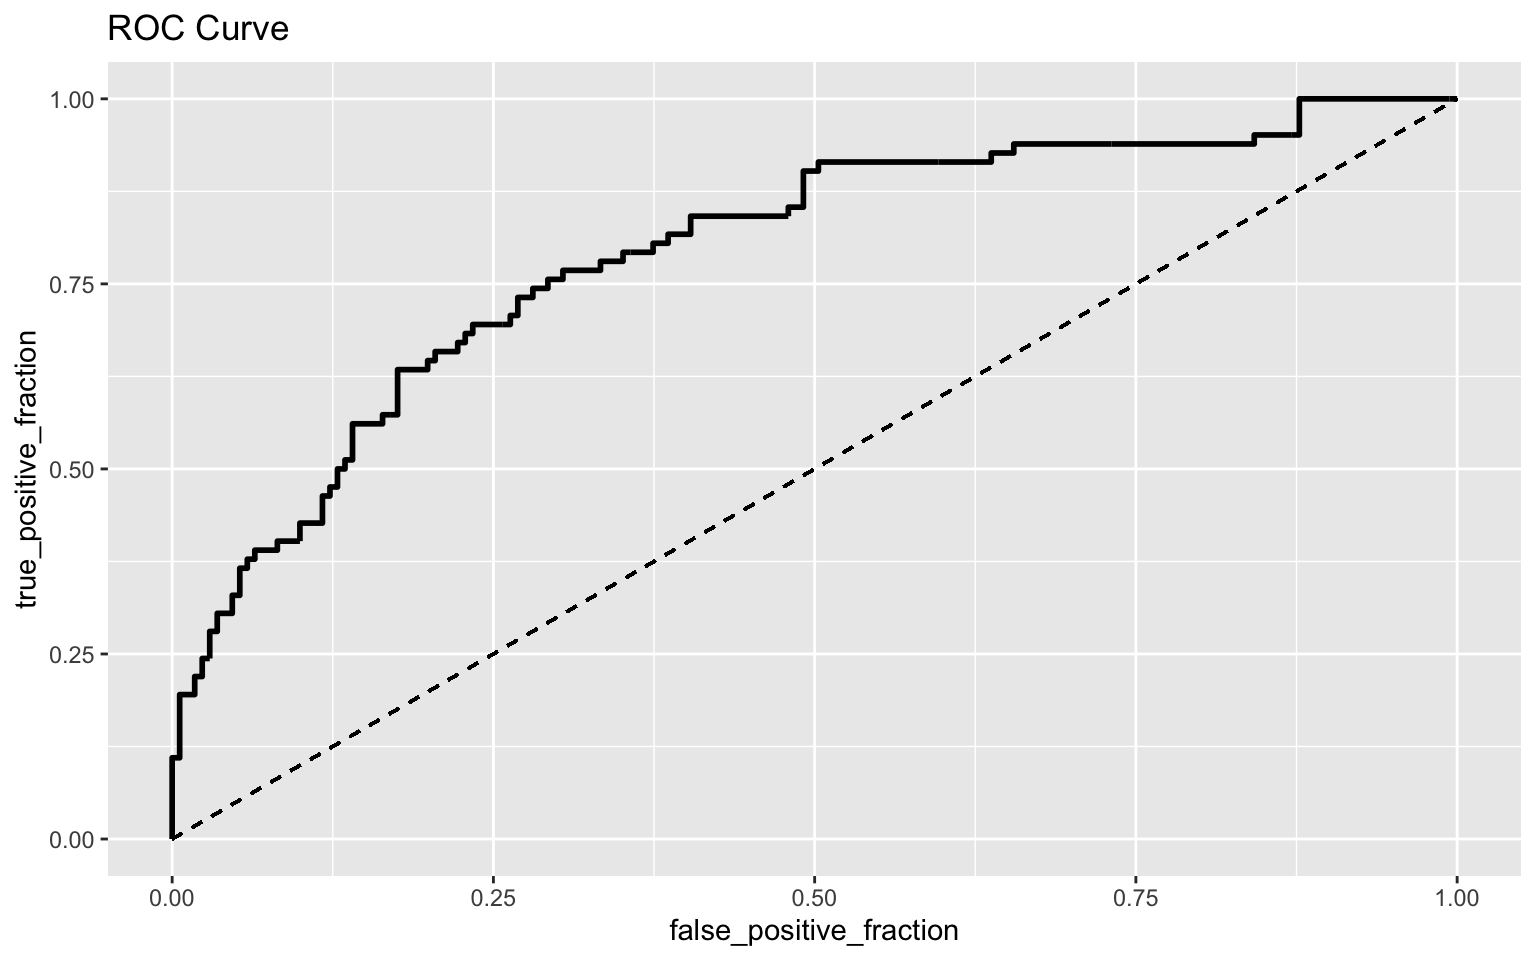
\includegraphics{project2_files/figure-latex/unnamed-chunk-7-2} \end{center}

\begin{Shaded}
\begin{Highlighting}[]
\CommentTok{#AUC Calculation}
\KeywordTok{calc_auc}\NormalTok{(ROCplot)}
\end{Highlighting}
\end{Shaded}

\begin{verbatim}
##   PANEL group       AUC
## 1     1    -1 0.7925403
\end{verbatim}

\begin{Shaded}
\begin{Highlighting}[]
\CommentTok{#10-Fold CV}
\KeywordTok{set.seed}\NormalTok{(}\DecValTok{1234}\NormalTok{)}
\NormalTok{k=}\DecValTok{10}

\NormalTok{data1<-joindata_log[}\KeywordTok{sample}\NormalTok{(}\KeywordTok{nrow}\NormalTok{(joindata_log)),] }
\NormalTok{folds<-}\KeywordTok{cut}\NormalTok{(}\KeywordTok{seq}\NormalTok{(}\DecValTok{1}\OperatorTok{:}\KeywordTok{nrow}\NormalTok{(joindata_log)),}\DataTypeTok{breaks=}\NormalTok{k,}\DataTypeTok{labels=}\NormalTok{F) }

\NormalTok{diags<-}\OtherTok{NULL}
\ControlFlowTok{for}\NormalTok{(i }\ControlFlowTok{in} \DecValTok{1}\OperatorTok{:}\NormalTok{k)\{          }
\NormalTok{  train<-data1[folds}\OperatorTok{!=}\NormalTok{i,] }
\NormalTok{  test<-data1[folds}\OperatorTok{==}\NormalTok{i,]  }
  
\NormalTok{  truth<-test}\OperatorTok{$}\NormalTok{Urb_binary}
  
\NormalTok{  log_reg<-}\StringTok{ }\KeywordTok{glm}\NormalTok{(Urb_binary }\OperatorTok{~}\StringTok{ }\NormalTok{limitedaccessfoodrate}\OperatorTok{+}\NormalTok{Household.Income,}
                \DataTypeTok{data=}\NormalTok{train, }
                \DataTypeTok{family=}\StringTok{"binomial"}\NormalTok{)}
\NormalTok{  probs<-}\StringTok{ }\KeywordTok{predict}\NormalTok{(log_reg, }\DataTypeTok{type =} \StringTok{"response"}\NormalTok{, }\DataTypeTok{newdata=}\NormalTok{test)}
  
\NormalTok{  diags<-}\KeywordTok{rbind}\NormalTok{(diags,}\KeywordTok{class_diag}\NormalTok{(probs,truth))}
\NormalTok{\}}
\KeywordTok{summarize_all}\NormalTok{(diags,mean,}\DataTypeTok{na.rm=}\OtherTok{TRUE}\NormalTok{)}
\end{Highlighting}
\end{Shaded}

\begin{verbatim}
##         acc      sens      spec       ppv       auc
## 1 0.7312308 0.4194805 0.8875317 0.6244048 0.7852403
\end{verbatim}

\emph{The odds of urbanization with a limited food access rate of zero
and a household income of zero is 0.002087343. Controlling for household
income, for every one additional unit increase in the rate of limited
access to food, the odds of urbanization decrease by a factor of
0.993745502, but this does not have a significant negative impact.
Controlling for limited access to food rate, household income has a
significant positive impact on the odds of urbanization. Controlling for
limited access to food rate, for every one additional unit of household
income,the odds of urbanization increase by a factor of 1.000109233.}

\emph{The accuracy of the model was reported to be 0.743083, which means
that true results of classification, either positive or negative are
reported 74.31\% of the time for the classification of a county as urban
or rural. The sensitivity was reported to be 0.4146341, which means that
the true positive rate of counties being identified as urban happened
41.46\% of the time. The specificity was reported to be 0.9005848,
meaning that the true negative rate of counties being identified as
rural happened 90.06\% of the time. The precision of the model was
0.6666667, meaning that this is the proportion of counties classified as
urban that actually are urban in reality.}

\emph{The ROC curve above shows the tradeoff between sensitivity and
specificity, and the AUC is a reflection of the summarization of those
values. We can see that as the true positive rate increases, the false
positive rate increases as well. The calculation of the AUC from the ROC
plot gave a value of 0.7925403, which falls within the ``fair'' range
for how well the model of the rate of limited access to food and
household income predicts the data of urbanization classification.}

\emph{A 10-fold cross validation was done, and the average out-of-sample
accuracy was reported to be 0.7274744, which means that true results,
either positive or negative are reported 72.75\% of the time for the
classification of a county as urban or rural. The sensitivity was
reported to be 0.4075536, which means that the true positive rate of
counties being identified as urban happened only 40.76\% of the time.
The specificty was reported to be 0.8796805, which means that correct
identification of rural counties happened 87.97\% of the time. The PPV
was reported to be 0.6665476, meaning that this is the proportion of
counties classified as urban that actually are urban in reality. The AUC
of the model is 0.7722236, which falls in the classification of ``fair''
for how well the model predicts the data.}

\#LASSO and CV

\begin{Shaded}
\begin{Highlighting}[]
\KeywordTok{library}\NormalTok{(glmnet)}
\NormalTok{joindata_nona<-joindata_log}\OperatorTok\KeywordTok{drop_na}\NormalTok{()}\OperatorTok\KeywordTok{select}\NormalTok{(}\OperatorTok{-}\KeywordTok{c}\NormalTok{(County, }
\NormalTok{  foodinsecurerate_c, costpermeal_c, urbanization))}
\NormalTok{y<-}\KeywordTok{as.matrix}\NormalTok{(joindata_nona}\OperatorTok{$}\NormalTok{Urb_binary)}
\NormalTok{x<-}\KeywordTok{model.matrix}\NormalTok{(Urb_binary}\OperatorTok{~}\NormalTok{.,}\DataTypeTok{data=}\NormalTok{joindata_nona)[,}\OperatorTok{-}\DecValTok{1}\NormalTok{]}
\KeywordTok{head}\NormalTok{(x)}
\end{Highlighting}
\end{Shaded}

\begin{verbatim}
##   lifeexpectancy diabeticrate foodinsecurerate limitedaccessfoodrate
## 1           73.8           11               19                    15
## 2           76.8            9                9                    12
## 3           76.3           14               20                    11
## 4           76.9           14               16                    20
## 5           77.0           11               15                     5
## 6           72.4           11               14                    20
##   free_reduced_lunch_percent costpermeal Household.Income uninsuredchildrenrate
## 1                         61        2.75            42412                    11
## 2                         42        2.94            63451                    12
## 3                         66        2.94            45318                    10
## 4                         56        2.95            46970                    13
## 5                         32        2.83            58311                    13
## 6                         51        3.06            55337                    12
##   border_statusNon-Border childfoodinsecurityrate
## 1                       1                   0.234
## 2                       1                   0.184
## 3                       1                   0.253
## 4                       1                   0.263
## 5                       1                   0.201
## 6                       1                   0.203
\end{verbatim}

\begin{Shaded}
\begin{Highlighting}[]
\NormalTok{cv<-}\KeywordTok{cv.glmnet}\NormalTok{(x,y, }\DataTypeTok{family=}\StringTok{"binomial"}\NormalTok{)}
\NormalTok{lasso<-}\KeywordTok{glmnet}\NormalTok{(x,y,}\DataTypeTok{lambda=}\NormalTok{cv}\OperatorTok{$}\NormalTok{lambda}\FloatTok{.1}\NormalTok{se)}
\KeywordTok{coef}\NormalTok{(lasso)}
\end{Highlighting}
\end{Shaded}

\begin{verbatim}
## 11 x 1 sparse Matrix of class "dgCMatrix"
##                                       s0
## (Intercept)                 0.0690545319
## lifeexpectancy              .           
## diabeticrate                .           
## foodinsecurerate            .           
## limitedaccessfoodrate       .           
## free_reduced_lunch_percent  .           
## costpermeal                 .           
## Household.Income            0.0000142346
## uninsuredchildrenrate      -0.0359355608
## border_statusNon-Border     .           
## childfoodinsecurityrate     .
\end{verbatim}

\begin{Shaded}
\begin{Highlighting}[]
\CommentTok{#10-fold CV}
\KeywordTok{set.seed}\NormalTok{(}\DecValTok{1234}\NormalTok{)}
\NormalTok{k=}\DecValTok{10}
\NormalTok{data <-}\StringTok{ }\NormalTok{joindata_nona }\OperatorTok\StringTok{ }\NormalTok{sample_frac}
\NormalTok{folds <-}\StringTok{ }\KeywordTok{ntile}\NormalTok{(}\DecValTok{1}\OperatorTok{:}\KeywordTok{nrow}\NormalTok{(data),}\DataTypeTok{n=}\DecValTok{10}\NormalTok{)}
\NormalTok{diags<-}\OtherTok{NULL}
\ControlFlowTok{for}\NormalTok{(i }\ControlFlowTok{in} \DecValTok{1}\OperatorTok{:}\NormalTok{k)\{}
\NormalTok{train <-}\StringTok{ }\NormalTok{data[folds}\OperatorTok{!=}\NormalTok{i,]}
\NormalTok{test <-}\StringTok{ }\NormalTok{data[folds}\OperatorTok{==}\NormalTok{i,] }
\NormalTok{truth <-}\StringTok{ }\NormalTok{test}\OperatorTok{$}\NormalTok{Urb_binary}
\NormalTok{fit <-}\StringTok{ }\KeywordTok{glm}\NormalTok{(Urb_binary}\OperatorTok{~}\NormalTok{uninsuredchildrenrate}\OperatorTok{+}\NormalTok{Household.Income,}\DataTypeTok{data=}\NormalTok{train,}
           \DataTypeTok{family=}\StringTok{"binomial"}\NormalTok{)}
\NormalTok{probs <-}\StringTok{ }\KeywordTok{predict}\NormalTok{(fit, }\DataTypeTok{newdata=}\NormalTok{test, }\DataTypeTok{type=}\StringTok{"response"}\NormalTok{)}
\NormalTok{diags<-}\KeywordTok{rbind}\NormalTok{(diags,}\KeywordTok{class_diag}\NormalTok{(probs,truth))}
\NormalTok{\}}
\NormalTok{diags}\OperatorTok\KeywordTok{summarize_all}\NormalTok{(mean)}
\end{Highlighting}
\end{Shaded}

\begin{verbatim}
##         acc      sens      spec      ppv       auc
## 1 0.8179348 0.6327922 0.9250668 0.825873 0.8799389
\end{verbatim}

\emph{The LASSO regression retained Household Income and Rate of
Uninsured Children as the variables that were the best predictors for
Urban classification. The 10-fold CV performed on the binary Urban
classification variable gave an out-of-sample accuracy of 0.8269928,
which is greater than the out-of-sample accuracy in the logisitic
regression, which was 0.7274744. The AUC from the 10-fold CV for the
LASSO was 0.874748 which is really good, as opposed to an AUC of
0.7722236 for the logistic regression, which is fair. This means that
the LASSO regression performs better than a logisitic regression at
predicting true results, either positive or negative for the
classification of a county as urban or rural, by reducing overfitting of
the model.}

\end{document}
